\chapter{Implementación: compilador de CABS a ABS}

Una vez llegados a este punto del trabajo, podemos quedar convencidos de lo interesante que puede ser contar con una implementación real de un compilador de CABS a ABS. Dicha implementación se encuentra disponible en un repositorio auxiliar alojado en \url{https://github.com/MaSteve/cabs}\\

En este capítulo, resumiremos el funcionamiento del compilador desarrollado comentando brevemente las librerías empleadas para este fin.

\section{Introducción a los procesadores de lenguaje}

La historia de los compiladores se remonta a los años 50 del siglo pasado. En aquella época, la compilación de programas consistía en sustituir las líneas de un lenguaje de alto nivel por el código de las rutinas a las que hacían referencia.\\

En torno a esos años y en la siguiente década, se establecieron las bases para la actual teoría de autómatas. Los lenguajes formales quedan clasificados por la jerarquía de Chomsky en función de su expresividad. Los primeros lenguajes de programación empiezan a surgir moviendose en el ámbito de las gramáticas incontextuales, que son aquellas que se pueden procesar con un autómata con pila.\\

Es en esta categoría donde podemos encontrar a la mayoría de lenguajes de programación. En concreto, se buscan aquellos subconjuntos de gramáticas en los que se puede garantizar que existe un reconocedor o autómata determinista. Algunos ejemplos de gramáticas son la $LL(k)$, la $LR(k)$ y la $LALR(k)$.\\

Puede decirse que la función actual de un compilador es la de traducir entre distintos lenguajes basandose en una teoría formal y preservando una cierta corrección entre los lenguajes de origen y destino. Las fases por las que pasa un compilador son las siguientes:
\begin{itemize}
\item Front-end o fase de análisis: que se compone a su vez en
  \begin{itemize}
  \item Análisis léxico: a partir del código de origen se extraen los distintos elementos léxicos o tokens que lo componen, por ejemplo, las palabras reservadas del lenguaje, los nombres de variables, etc.
  \item Análisis sintáctico: usando los token del análisis léxico, mediante el uso de un autómata determinista que reconozca la gramática del lenguaje, se crea un árbol de sintaxis abstracta en cuyos nodos podemos encontrar las piezas lógicas que componen nuestro programa, por ejemplo, las asignaciones de variables, la declaración de funciones, etc.
  \item Análisis estático: en esta fase se analizan los identificadores usados en el programa, en busca de usos ilícitos como en el caso de las asignaciones en variables no declaradas, y los tipos de las expresiones que permiten descartar programas con errores. De este proceso se obtiene una tabla de símbolos que puede ser de ayuda en la traducción final del código.
  \end{itemize}
\item Back-end o fase de traducción: a partir del árbol de sintaxis abstracta y del resto de estructuras obtenidas en la etapa anterior, el compilador genera un código objeto entendible para la máquina o interprete para el que está destinado. En esta etapa también se pueden llevar a cabo algunas optimizaciones, pero hablar de ello no es nuestro objetivo.
\end{itemize}

\section{JLex}

JLex\footnote{\url{https://www.cs.princeton.edu/~appel/modern/java/JLex/current/manual.html}} es un generador de analizadores léxicos en java desarrollado en la Universidad de Princeton. A partir de una especificación de los tokens de un lenguaje, JLex genera un autómata capaz de reconocerlos recogido en una clase de Java.\\

El automata empleado en los analizadores léxicos es un autómata finito determinista, categoría en la que se encuentran los reconocedores de los lenguajes formales más básicos conocidos como lenguajes regulares.\\

La especificación del analizador léxico de CABS se puede encontrar en el archivo {\verb parser.lex } dentro del paquete {\verb parser }. A su vez, dentro de este paquete se encuentran la clase {\verb Yytoken }, que será el tipo de objeto manipulado por el analizador sintáctico, y el archivo {\verb Yylex.java }, con las clases asociadas al autómata finito determinista.\\

\begin{figure}[h]
  \centering
  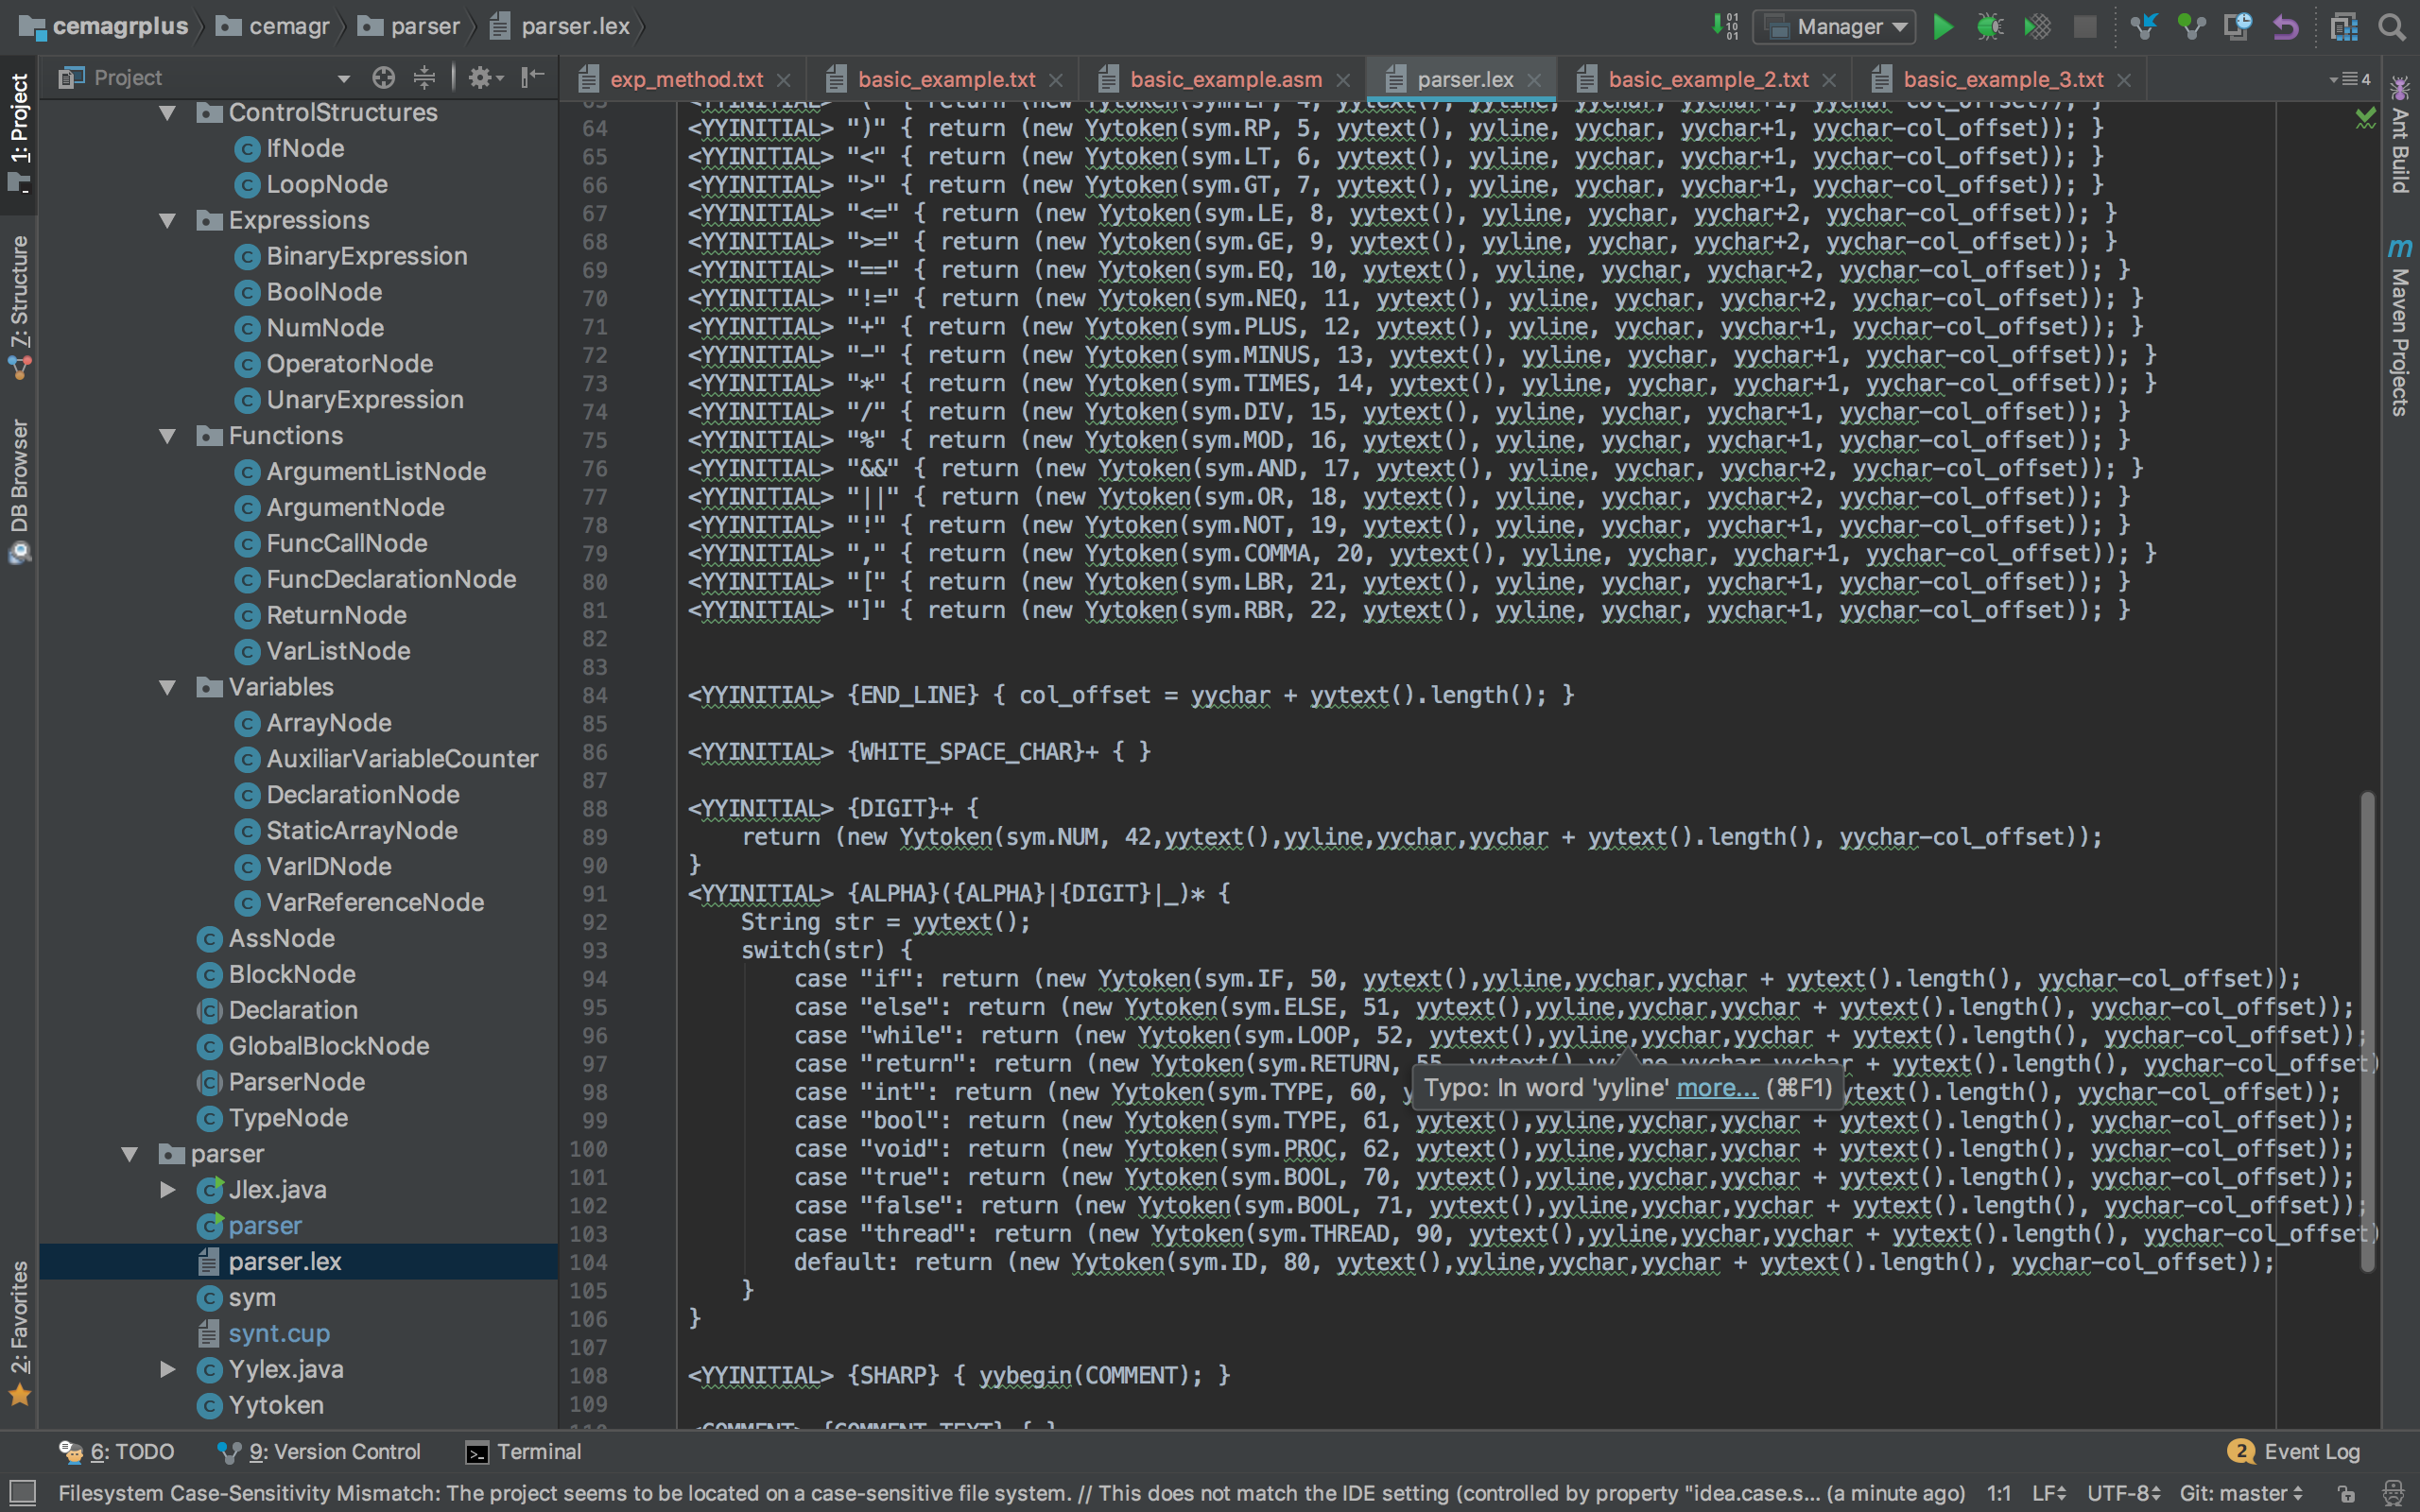
\includegraphics[scale=0.36]{jlex.png}
  \caption{Captura de las reglas para la generación del lexer.}
\end{figure}
